\uuid{tPb8}
\chapitre{Application linéaire}
\sousChapitre{Autre}
\titre{ Classification linéaire par un perceptron }
\theme{réseaux de neurones}
\auteur{ Maxime NGUYEN }
\datecreate{2024-11-17}
\organisation{ AMSCC }

\contenu{
	
	\question{ 

Décrire un perceptron qui permet de réaliser la classification entre les points bleus et les points rouges comme dans le graphique ci-dessous. Justifier.



\begin{center}
	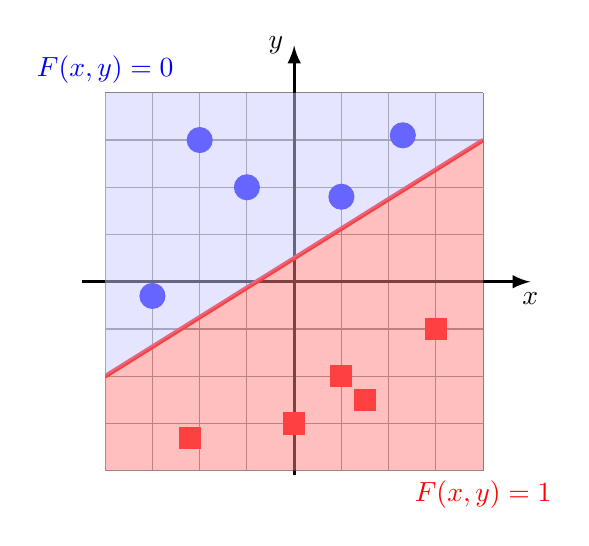
\begin{tikzpicture}[scale=0.6]
		\tikzstyle{rouge} = [fill,rectangle,red,scale=1.2];
		\tikzstyle{bleu} = [fill,circle,blue] ;
		
		
		\draw[gray] (-4,-4) grid ++(8,8);
		\draw[->,>=latex, very thick,black] (-4.5,0)--(5,0) node[below] {$x$};
		\draw[->,>=latex, very thick, black] (0,-4.1)--(0,5) node[left] {$y$};
		
		
		\foreach \x/\y in {-2/3,-1/2,-3/-0.3,1/1.8,2.3/3.1}{
			\node[bleu] at (\x,\y) {};
		}
		\foreach \x/\y in {1/-2,3/-1,1.5/-2.5,0/-3,-2.2/-3.3}{
			\node[rouge] at (\x,\y) {};
		}
		
		
		\begin{scope}[even odd rule]
			\clip (-4,-4) rectangle (4,4);
			\draw[red,ultra thick] (4,3) -- (-4,-2);
			\fill[red!50,opacity=0.5] (4,3) -- (4,-4) --(-4,-4)--(-4,-2) -- cycle;
			\fill[blue!20,opacity=0.5] (4,3) -- (4,4) --(-4,4)--(-4,-2) -- cycle;
			
			
		\end{scope}
		
		
		\node[scale=1,red,below] at (4,-4) {$F(x,y)=1$};
		\node[scale=1,blue,above] at (-4,4) {$F(x,y)=0$};
		%\node[red,below] at (-1,-4) {$y=8x+4$};
		
		
	\end{tikzpicture}
\end{center}
}

\reponse{ We want to separate the plane into to half planes. One can consider the red line defined by $y=5x/8+1/2$ that is $5x-8y+4 = 0$ or another line which separates as well, for example $5x-8y=0$.  So this perceptron can fit to this problem.
	
	
	\begin{center}
		\begin{tikzpicture}[scale=0.5]
			\draw[thick,fill=black!10] (0,0) circle (2);
			\node at (150:9) {$x$};
			\node at (190:9) {$y$};
			\draw[ultra thick]  (150:3) -- (150:8)node[pos=0.3,above]{$5$};;
			\draw[ultra thick]  (190:3) -- (190:8) node[pos=0.3,above]{$-8$};
			\draw[-o,ultra thick]  (210:3) -- (210:8) node[pos=0.3,above]{$4$};
			\draw[->,>=latex,ultra thick] (0:3) --  (8,0) node[right] {};
			\node[below right] at (-15:3) {$H$};
		\end{tikzpicture}  
	\end{center}
	
	
}
}
